\section{Bifurcations}


\begin{figure}
    \centering
    \begin{subfigure}{0.4\textwidth}
        \centering
        \includegraphics[width=\textwidth]{60_Final/2D_Regions_Whole/result-halved.png}
        \caption{Complete Parameter Region}
        \label{fig:final.regions.whole.halved}
    \end{subfigure}
    \begin{subfigure}{0.4\textwidth}
        \centering
        \includegraphics[width=\textwidth]{60_Final/2D_Regions_CandD16/result-halved.png}
        \caption{Only showing $C_{16}$ and $D_{16}$}
        \label{fig:final.regions.CandD16.halved}
    \end{subfigure}
    \caption{2D Period Regions of Halved Final Model}
\end{figure}

\todo{what bifurcations (which borders) in type A / type B regions}

\subsection{``Type'' A Parameter Regions}

\subsubsection{$C_{16}^\uparrow$}

\begin{figure}
    \centering
    \begin{subfigure}{0.4\textwidth}
        \centering
        \includegraphics[width=\textwidth]{60_Final/1D_Bif_LCU16/result.png}
        \caption{Complete}
        \label{fig:bifurcation.C.up}
    \end{subfigure}
    \begin{subfigure}{0.4\textwidth}
        \centering
        \includegraphics[width=\textwidth]{60_Final/1D_Bif_LCU16_Zoomed/result.png}
        \caption{Zoomed in at Border $\A\B$}
        \label{fig:bifurcation.C.up.zoomed}
    \end{subfigure}
    \caption{1D Bifurcation Diagram of $C_{16}^\uparrow$}
\end{figure}

\subsubsection{$C_{16}^\rightarrow$}

\begin{figure}
    \centering
    \begin{subfigure}{0.4\textwidth}
        \centering
        \includegraphics[width=\textwidth]{60_Final/1D_Bif_LCR16/result.png}
        \caption{Complete}
        \label{fig:bifurcation.C.right}
    \end{subfigure}
    \begin{subfigure}{0.4\textwidth}
        \centering
        \includegraphics[width=\textwidth]{60_Final/1D_Bif_LCR16_Zoomed/result.png}
        \caption{Zoomed in at Border $\B\C$}
        \label{fig:final.bifurcation.C.right.zoomed}
    \end{subfigure}
    \caption{1D Bifurcation Diagram of $C_{16}^\rightarrow$}
\end{figure}

\subsubsection{$C_{16}^\downarrow$}

\begin{figure}
    \centering
    \begin{subfigure}{0.4\textwidth}
        \centering
        \includegraphics[width=\textwidth]{60_Final/1D_Bif_LCD16/result.png}
        \caption{Complete}
        \label{fig:bifurcation.C.down}
    \end{subfigure}
    \begin{subfigure}{0.4\textwidth}
        \centering
        \includegraphics[width=\textwidth]{60_Final/1D_Bif_LCD16_Zoomed/result.png}
        \caption{Zoomed in at Border $\A\B$}
        \label{fig:final.bifurcation.C.down.zoomed}
    \end{subfigure}
    \caption{1D Bifurcation Diagram of $C_{16}^\downarrow$}
\end{figure}

\subsubsection{$C_{16}^\leftarrow$}

\begin{figure}
    \centering
    \begin{subfigure}{0.4\textwidth}
        \centering
        \includegraphics[width=\textwidth]{60_Final/1D_Bif_LCL16/result.png}
        \caption{Complete}
        \label{fig:bifurcation.C.left}
    \end{subfigure}
    \begin{subfigure}{0.4\textwidth}
        \centering
        \includegraphics[width=\textwidth]{60_Final/1D_Bif_LCL16_Zoomed/result.png}
        \caption{Zoomed in at Border $\B\C$}
        \label{fig:final.bifurcation.C.left.zoomed}
    \end{subfigure}
    \caption{1D Bifurcation Diagram of $C_{16}^\leftarrow$}
\end{figure}

\subsection{``Type B'' Parameter Regions}
